\documentclass[tikz,border=10pt]{standalone}
\usetikzlibrary{arrows.meta,positioning,calc}
\begin{document}
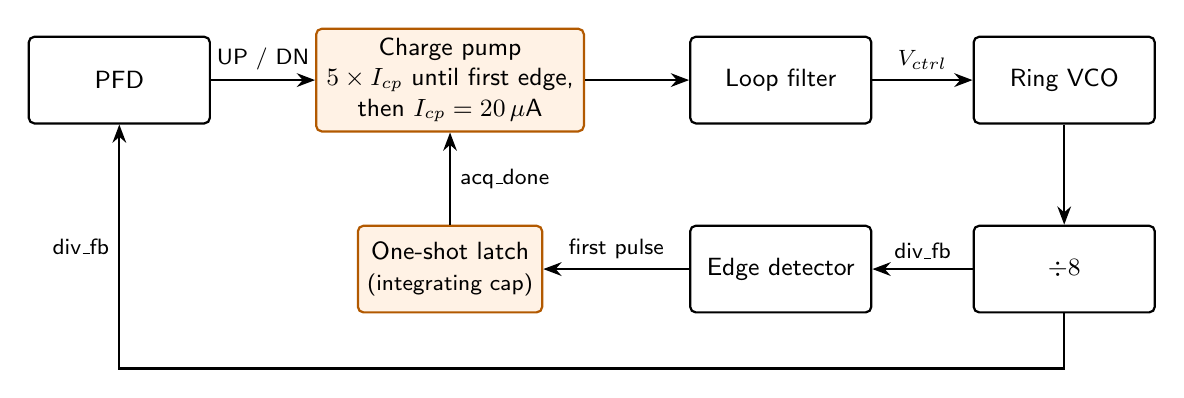
\begin{tikzpicture}[
  >=Stealth, thick, font=\sffamily\small,
  blk/.style={draw, rounded corners=2pt, minimum height=1.1cm, minimum width=2.3cm, align=center, fill=white},
  hl/.style={blk, fill=orange!10, draw=orange!70!black},
  lab/.style={font=\sffamily\footnotesize, align=center}
]
\node[blk] (pfd) at (0,0) {PFD};
\node[hl, minimum width=3.4cm] (cp) at (4.2,0) {Charge pump\\$5\times I_{cp}$ until first edge,\\then $I_{cp}=20\,\mu$A};
\node[blk] (lf) at (8.4,0) {Loop filter};
\node[blk] (vco) at (12,0) {Ring VCO};
\node[blk] (div) at (12,-2.4) {$\div 8$};
\node[blk] (edge) at (8.4,-2.4) {Edge detector};
\node[hl] (latch) at (4.2,-2.4) {One-shot latch\\{\footnotesize (integrating cap)}};

\draw[->] (pfd) -- node[above,lab]{UP / DN} (cp);
\draw[->] (cp) -- (lf);
\draw[->] (lf) -- node[above,lab]{$V_{ctrl}$} (vco);
\draw[->] (vco) -- (div);
\draw[->] (div) -- node[above,lab]{div\_fb} (edge);
\draw[->] (edge) -- node[above,lab]{first pulse} (latch);
\draw[->] (latch) -- node[right,lab]{acq\_done} (cp);
\draw[->] (div.south) -- ++(0,-0.7) -| node[pos=0.75,left,lab]{div\_fb} (pfd.south);
\end{tikzpicture}
\end{document}
